\section{Different Poisson solvers}
\label{SEC_SCARC_poisson}

Subsequently the different Poisson solvers available in FDS are described. They are based on different combinations of global/local and structured/unstructured discretizations.


\subsection{Mesh-wise FFT}

Spectral solvers like the {\it Fast Fourier Transformation} (FFT) belong to the class of direct solvers and exploit a very special property of the underlying Poisson problem, namely that sine and cosine functions are eigenvectors of the Laplace operator. They expand the solution as a Fourier series which can be quickly performed at rather low complexity. 

In practice, FFT-solvers have proven to be highly efficient and are used in many different fields of application. However, they are restricted to structured grids which may impede their use for complex geometries.

As described in detail in the FDS Technical Guide~\cite{McGrattan:2018:TG}, the pressure equation (\ref{EQ_pressure}) is obtained from the momentum equation by a sequence of substitutions and simplifications. The major advantage of this derivation is that it finally leads to a system of equations which has constant coefficients (i.e.\ is separable). In its default version FDS is based on the use of local structured discretizations where the single meshes are of cubic shape with uniform grid resolutions each. Correspondingly, a highly optimized FFT solver for regular grids from the package CRAYFISHPAK~\cite{Sweet::Crayfishpak} is used as the default Poisson solver in FDS.

For a single-mesh application only one globally acting FFT-method is performed which has proven to be extremely powerful and unbeatably fast over the past years since its highly recursive character extremely well captures the fast global information transfer within the only grid used. For multi-mesh applications, however, there is no longer one global rectangular discretization, but only a collection of local ones as explained above, such that the global connectivity is split off. Now, every sub-mesh performs its own local FFT to compute an exact solution to the related local Poisson problem, see Figure \ref{FIG_local_ffts}. 
The global solution is then composed from the local ones.
\begin{figure}[h]
\begin{center}
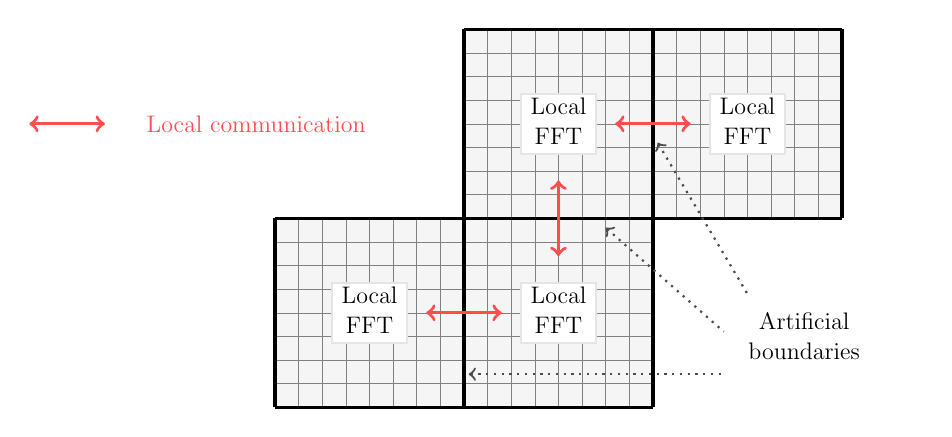
\begin{tikzpicture}
[
scale=0.6,
every node/.style={scale=0.6},
Background/.style={rectangle,draw=black!04,fill=black!04, thin, minimum size = 4 cm},
Obstruction/.style={rectangle,draw=black!70,fill=black!40, very thick, minimum size=1cm},
Finegrid/.style={step=0.5cm,gray,very thin},
Thickline/.style={-,draw=black!100,fill=black!02, very thick},
Thinline/.style={draw=black!100,fill=black!02, very thin},
Ball/.style={circle, draw=black!40, fill=red!20, thin, minimum size=3.5mm},
Circle/.style={circle,draw=black!40,fill=black!06,thin,minimum size=35.5mm},
Rectangle/.style={rectangle,draw=black!10,fill=white,inner xsep=0pt, inner ysep=0pt,},
Box/.style= {very thin, rectangle, inner xsep=10pt, inner ysep=10pt,},
ComArrow/.style= {<->,very thick, draw=red!70,},
DotArrow/.style= {<-, thick, dotted, draw=black!70,},
]

\node[Background] at (  2,2) {};
\node[Background] at (  6,2) {};
\node[Background] at (  6,6) {};
\node[Background] at (10,6) {};

\node[Obstruction] at (2,2) {};

\draw[Finegrid] (0,0) grid (  8,4);
\draw[Finegrid] (4,4) grid (12,8);

\draw[Thickline] (0,0)--(  8,0);
\draw[Thickline] (4,8)--(12,8);
\draw[Thickline] (0,4)--(  4,4);
\draw[Thickline] (8,4)--(12,4);

\draw[Thickline] (  0,0)--(  0,4);
\draw[Thickline] (  4,8)--(12,8);
\draw[Thickline] (  4,4)--(  4,8);
\draw[Thickline] (  8,0)--(  8,4);
\draw[Thickline] (12,4)--(12,8);

\draw[Thickline] (4,0)--(4,4);
\draw[Thickline] (4,4)--(8,4);
\draw[Thickline] (8,4)--(8,8);

\node[Rectangle] at (  2,2.0) {\Large \begin{tabular}{c} Local \\ FFT\end{tabular}};
\node[Rectangle] at (  6,2.0) {\Large \begin{tabular}{c} Local \\ FFT\end{tabular}};
\node[Rectangle] at (  6,6.0) {\Large \begin{tabular}{c} Local \\ FFT\end{tabular}};
\node[Rectangle] at (10,6.0) {\Large \begin{tabular}{c} Local \\ FFT\end{tabular}};

\draw[ComArrow](3.2,2)--(4.8,2);
\draw[ComArrow](6,3.2)--(6,4.8);
\draw[ComArrow](7.2,6)--(8.8,6);

\draw [DotArrow] (8.1,5.6) -- (10.0,2.4);
\draw [DotArrow] (7.0,3.8) -- (  9.5,1.6);
\draw [DotArrow] (4.1,0.7) -- (  9.5,0.7);

\node [Box] (box) at (11.2,1.5){%
    \begin{minipage}{0.36\textwidth}
    \begin{center}
        {\Large Artificial \\[1ex]
           boundaries}
    \end{center}
    \end{minipage}};

\draw[ComArrow](-5.2,6)--(-3.6,6);
\node [Box,red!70] (box) at (-0.4,6){%
    \begin{minipage}{0.56\textwidth}
    \begin{center}
        {\Large Local communication}
    \end{center}
    \end{minipage}};

\end{tikzpicture}

\caption[Mesh-wise FFT-method]{Mesh-wise FFT-method for the {\ct poisson2d} geometry: First each mesh performs its own local FFT method, which requires data exchanges between neighboring meshes to define the boundary conditions along the new artificial boundaries. Then the global solution results from the composition of the local solutions.}
\label{FIG_local_ffts}
\end{center}
\end{figure}

\vspace{-0.3cm}
A drawback associated with this approach is that the mathematical solvability of the local problems requires the definition of appropriate boundary conditions all over the local boundary. This particularly includes the cells along the new artificial boundaries between the meshes, but the correct boundary conditions are not known there at all. Instead, they are only approximately defined as Dirichlet boundary values, consisting of the mean values of neighboring cells in adjacent meshes taken from the last time step, which may lead to losses of accuracy.

On the other hand, this strictly locally oriented approach possesses an extremely high parallel efficiency because the required values for the definition of the boundary data have already been computed in the preceding time step and the exchange of the internal boundary values only requires next-neighbor communications which can be performed with great computational efficiency on today's parallel architectures.


There might be another disadvantage associated with this procedure:
As already described, the most fundamental characteristic of the pressure equation (\ref{EQ_pressure})  is a very fast propagation speed for information. Only a single time step may suffice to spread new information over the whole computational domain, i.e.\ local effects or perturbations have immediate impact on the overall solution. 
Due to the purely local character of the mesh-wise FFT solver, however, new information can only be transferred mesh-by-mesh, successively using the data exchanges between adjacent meshes  as illustrated in Figure \ref{FIG_mesh_wise_transfer}.
\vspace{-0.2cm}
\begin{center}
\begin{figure}[ht]
\begin{minipage}{4.3cm}
\input{\tikzPath/multi_pipe_fft_cycle1.tex}
\end{minipage}
\begin{minipage}{3.9cm}
\input{\tikzPath/multi_pipe_fft_cycle2.tex}
\end{minipage}
\begin{minipage}{3.9cm}
\input{\tikzPath/multi_pipe_fft_cycle3.tex}
\end{minipage}
\begin{minipage}{3.9cm}
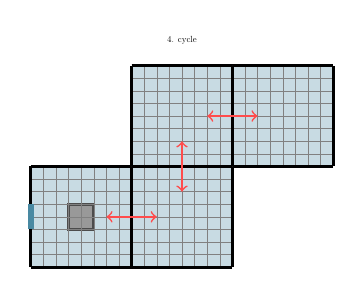
\begin{tikzpicture}
[
scale=0.32,
every node/.style ={scale=0.32},
Background/.style={rectangle,draw=black!04,fill=black!04, thin, minimum size = 4 cm},
BackgroundInflow/.style={rectangle,draw=black!04,fill={rgb,255:red,73;green,137;blue,162},opacity=0.3, thin, minimum size = 4 cm},
Obstruction/.style={rectangle,draw=black!70,fill=black!40, very thick, minimum size=1cm},
Finegrid/.style={step=0.5cm,gray,very thin},
Thickline/.style={-,draw=black!100,fill=black!02, very thick},
Thinline/.style={draw=black!100,fill=black!02, very thin},
Inflow/.style={-,draw={rgb,255:red,73;green,137;blue,162},line width=0.8mm},
Inarrow/.style={->,draw={rgb,255:red,73;green,137;blue,162},thin},
Outflow/.style={-,draw=blue!60,,line width=0.8mm},
Ball/.style={circle, draw=black!40, fill=red!20, thin, minimum size=3.5mm},
Circle/.style={circle,draw=black!40,fill=black!06,thin,minimum size=35.5mm},
Rectangle/.style={rectangle,draw=black!10,fill=white,inner xsep=0pt, inner ysep=0pt,},
Box/.style= {very thin, rectangle, inner xsep=10pt, inner ysep=10pt,},
ComArrow/.style= {<->,semithick,draw=red!70},
]

\node[BackgroundInflow] at (2,2) {};
\node[BackgroundInflow] at (6,2) {};
\node[BackgroundInflow] at (6,6) {};
\node[BackgroundInflow] at (10,6) {};

\node[Obstruction] at (2,2) {};

\draw[Finegrid] (0,0) grid (8,4);
\draw[Finegrid] (4,4) grid (12,8);

\draw[Thickline] (0,0)--(8,0);
\draw[Thickline] (4,8)--(12,8);
\draw[Thickline] (0,4)--(4,4);
\draw[Thickline] (8,4)--(12,4);

\draw[Thickline] (0,0)--(0,4);
\draw[Thickline] (4,8)--(12,8);
\draw[Thickline] (4,4)--(4,8);
\draw[Thickline] (8,0)--(8,4);
\draw[Thickline] (12,4)--(12,8);

\draw[Thickline] (4,0)--(4,4);
\draw[Thickline] (4,4)--(8,4);
\draw[Thickline] (8,4)--(8,8);

\draw[Inflow]   (0,1.5)--(0,2.5);
%\draw[Inarrow]  (-1,1.6)--(-0.25,1.6);
%\draw[Inarrow]  (-1,2.0)--(-0.25,2.0);
%\draw[Inarrow]  (-1,2.4)--(-0.25,2.4);
%\draw[Outflow]  (12,4)--(12,8);

\draw[ComArrow](3.0,2)--(5.0,2);
\draw[ComArrow](6,3.0)--(6,5.0);
\draw[ComArrow](7.0,6)--(9.0,6);

\node [Box] (Box) at (6.0,9.0){{\HUGE 4. cycle}};

\end{tikzpicture}

\end{minipage}
\caption[Delayed information transfer of the mesh-wise FFT solver]{Delayed information transfer of the mesh-wise FFT solver for the {\ct poisson2d} geometry: New information can only be passed across the whole domain by successively using the next-neighbor communications between adjacent meshes.}
\label{FIG_mesh_wise_transfer}
\end{figure}
\end{center}

\vspace{-0.6cm}
This necessarily involves a time delay compared to the real physical propagation speed and brings dependencies on the number of subdomains into play.
The higher the number of subdomains and the associated artificial fragmentation of the global connectivity is, the stronger this effect may be with corresponding negative impacts on the accuracy and stability of the whole method.
Nevertheless, for small numbers of subdomains this effect has proven to be very weak and the efficiency of the local FFT-methodology mainly dominates.


Finally, the following possible difficulties must be taken into account: Although the pressure term $\cH$ is continuous at mesh interfaces, the finite-difference of its gradient is not such that the normal components of velocity may be different at mesh interfaces. Furthermore, as already described in the context of
the structured discretization type, the normal components of velocity may be non-zero towards solid internal boundaries, or in other words, the velocity field may penetrate into internal obstructions. 

In order to compensate these undesired effects an additional iterative correction strategy based on a {\it Direct Forcing Immersed Boundary Method}~\cite{Fadlun:2000} is used in FDS: In every time step the mesh-wise FFT algorithm is not only applied once but multiple times until a specified tolerance for the velocity error along internal obstructions and mesh interfaces has been reached. 
For both, the internal obstructions and the mesh interfaces, the required velocity tolerance and the maximum allowed number of pressure iterations can be specified by the quantities {\ct VELOCITY\_TOLERANCE} and {\ct  MAX\_PRESSURE\_ITERATIONS} 
in the {\ct \&PRES}-namelist. By default, a velocity tolerance of ``characteristic mesh size'' divided by 10 and a maximum of 10 iterations is used. 
%
Certainly, the increased number of mesh-wise FFT solutions leads to a higher computational effort. Nevertheless, for a multitude of cases, especially in case of  small mesh numbers or in steady-state like situations, only less pressure iterations are usually needed and convergence is achieved very quickly.

\begin{figure}[h]
\begin{center}
\input{\tikzPath/multi_pipe_fft_presite.tex}
\caption[Mesh-wise FFT-methods with pressure correction]{Repeated use of the mesh-wise FFT solver for the {\ct poisson2d} geometry: In the scope of a surrounding pressure iteration the local FFT's are performed multiple times until the error related to the normal components of the velocity field along mesh interfaces and internal obstructions has been driven below a specified velocity tolerance.}
\label{FIG_SCARC_local_ffts_ite}%TODO keine Ref
\end{center}
\end{figure}

Increasing the number of subdomains may worsen the convergence and accuracy behaviour associated with a noticeable increase of computational costs.
Particularly, for extended geometries with a large number of meshes (i.e.\ tunnels) and/or transient boundary conditions this purely local strategy may experience difficulties to reproduce the rapid propagation of information for elliptic problems fast enough. In particular, these situations make the development of alternative solution concepts appear necessary and have driven their development forward.

\subsection{\uglmat}
Within the framework of the Gaussian elimination algorithm, many direct algorithms rely on the ``lower-upper''-factorization of the system matrix, $LU = A$, 
with corresponding triangular matrices $L$ and $U$, see Fig.~\ref{FIG_SCARC_lu_decomposition}. 
The solution of the global system of equations  (\ref{EQ_SCARC_single_system}) can then simply be obtained using a forward substitution step, $Ly=b$, followed by a backward substitution step, $Ux=y$, which can be performed at low computational costs.
The solver \uglmat{} which is available as alternative Poisson solver in FDS is a representative of this methodology.
\begin{figure}[h]
\begin{center}
\begin{tikzpicture}
[ 
  every node/.style ={scale=0.35},
 ]
\tikzstyle{every path}=[draw, line width=0.3mm];
\def\bracket{
  \draw[-] (1,10) -| (0,0) -- (1,0);
  \draw[-] (9,10) -| (10,0) -- (9,0);
}
\def\basecoords{ 
    \coordinate (-v1) at (1,1);
    \coordinate (-v2) at (9,1);
    \coordinate (-v3) at (9,9);
    \coordinate (-v4) at (1,9);
}
\tikzset{pics/.cd,
  my square/.style={code={\basecoords\fill [#1] (-v1) rectangle (-v3);\bracket}},
  my trileft/.style={code={\basecoords\fill [#1] (-v2) -- (-v4) -- (-v1);\bracket}},
  my triright/.style={code={\basecoords\fill [#1] (-v2) -- (-v3) -- (-v4);\bracket}}
 }

\pic[local bounding box=A,scale=0.4]  at (0,0)                              {my square={opacity=0.3,gray} };
\pic[local bounding box=B,scale=0.4,right=2 cm of A.south east] {my trileft   ={opacity=0.3,gray}};
\pic[local bounding box=C,scale=0.4,right=2 cm of B.south east] {my triright ={opacity=0.3,gray}};

\node[scale=2] (a) at ($(A.east)!0.5!(B.west)$) {$=$};
\node[scale=2] (b) at ($(B.east)!0.5!(C.west)$) {$\times$};

\node[scale=2] (At) at ([shift={(80:0.5)}]$(A.north)$) {$A$};
\node[scale=2] (Bt) at ([shift={(80:0.5)}]$(B.north)$) {$L$};
\node[scale=2] (Ct) at ([shift={(80:0.5)}]$(C.north)$) {$U$};
\end{tikzpicture}

\end{center}
\caption{Decomposition of $A$ into a lower triangular matrix $L$ and an upper triangular matrix $U$.}
\label{FIG_SCARC_lu_decomposition}
\end{figure}

Based on a global unstructured discretization of the overall system of equations (\ref{EQ_SCARC_single_system}), \uglmat{} is able to compute the exact global solution up to machine precision. In particular, there are no errors along mesh interfaces and internal obstructions which is a major advantage of this approach. 
\uglmat{} is basically built on the use of the optimized {\tt CLUSTER\_SPARSE\_SOLVER} solver of the Intel\textsuperscript{\textregistered} Math Kernel Library which can be applied for structured and unstructured discretizations. 
Compared to the optimized CRAYFISHPAK-FFT solver, however, it turns out to be slower by a factor of about 2 when applied for the same structured grid computation.
Note, that \uglmat{} currently can only be used for non-overlapping, non-stretched meshes at the same refinement level.

A main disadvantage of this approach is that less benefit can be drawn from the aforementioned sparsity of the Poisson matrix $A$. Unfortunately, the $LU$-factorization process leads to {\it fill-in}, i.e.\ it produces non-zero entries in $L$ and $U$ where $A$ was zero before as illustrated in Figure \ref{FIG_SCARC_lu_memory_spy}. There, the sparsity patterns of the Poisson matrix $A$
and its respective lower triangular matrix $L$ are compared in case of a simple 3D-cube geometry with a refinement into $16^3$ cells which already leads to the very unequal ratio of about 27 thousand non-zeros for $A$ to about 1 million non-zeros for $L$.
If the 3D-cube is further refined from $16^3$ up to $128^3$ cells this ratio even worsens dramatically and $L$ requires about 238 times more memory than $A$. 

\begin{figure}[h]
\begin{center}
\includegraphics[width=0.32\textwidth]{\figPath/Spy_A.png}\qquad\qquad\qquad
\includegraphics[width=0.32\textwidth]{\figPath/Spy_L.png}\\
\end{center}
\caption[Sparsity patterns for the decomposition $A=LU$ in case of a refined 3D-cube with $16^3$ cells]{
Sparsity patterns for the decomposition $A=LU$ in case of a refined 3D-cube with $16^3$ cells:
(Left) Poisson matrix $A$ with about 27 thousand non-zeros; (Right) Lower triangular matrix $L$ with nearly 1 million non-zeros;
}
\label{FIG_SCARC_lu_memory_spy}
\end{figure}

Thus, the storage of $L$ can become prohibitively expensive which especially holds true in case of huge systems of equations with many millions of unknowns. 
For realistically large CFD-problems, the associated additional storage requirements may exceed the capacity of the available computing system in the worst case. Hence, when considering the computational efficiency of $LU$-methods for a given application the resulting fill-in is a decisive criterion.
All in all, the highly recursive, domain-spanning dependencies which have to be mapped in the $LU$-process
make an efficient parallelization towards higher number of meshes rather difficult and decrease the scalability properties of this class of methods. For smaller numbers of meshes, however, \uglmat{} can be a good alternative to the default FFT solver what needs to be tested in each individual case. As an example the {\ct dancing\_eddies} case from FDS Users's Guide can be considered.


\subsection{\scarc{}}
With the aim to combine the advantages of the above Poisson solvers and to best possibly avoid their disadvantages, the solver package \scarc{} was developed. In contrast to the upper two solvers FFT and \uglmat{}, which both belong to the class of direct solvers, \scarc{} is mainly based on iterative solution techniques.

While direct methods only require a single, but possibly very complex computational cycle to solve the system of equations exactly, iterative solvers perform multiple cycles producing a sequence of iterations which gradually improve an initial estimate of the solution until a predefined stopping criterion has been reached. 

The computational complexity associated with each cycle of iterative methods is comprehensively less compared to the respective single cycle of direct methods. Thus, in comparison to direct methods, iterative methods are faced with the crucial question of how many cycles are ultimately required to achieve convergence.

\subsubsection{Basic iteration with Schwarz preconditioning}
The simplest form of an iterative methods is the so-called {\it basic iteration}, 
\be 
  x^k = x^{k-1} + B\, (b - Ax^{k-1})\,, 
\label{EQ_basic_iteration}
\ee
with iteration vectors $x^k, x^{k-1} \in \mathbb{R}^{n}$  and a {\it preconditioning matrix} matrix $B \in \mathbb{R}^{n \times n}$, 
which is used to increase the convergence speed by best possibly exploiting special knowledge of the underlying structure. Note, that $B$ does not need to be built explicitly, but is only defined by its action. 

Because the convergence properties of ({\ref{EQ_basic_iteration}) itself are poor, more efficient generalizations are typically used such as the {\it preconditioned conjugate gradient method} (CG) and the {\it geometric multigrid method}  (MG) which are able to significantly speed up convergence. For more detailed information on iterative methods please see Hackbusch \cite{Hackbusch:1994} or Saad \cite{Saad:2003}.

Usually, iterative methods are easier to implement than direct ones, because they can be reduced to a series of core components such as matrix-vector multiplications, scalar-products or linear-combinations of vectors, for which highly optimized program packages can be used, e.g.\ BLAS~\cite{Dongarra:1998, Dongarra:2002}.
Because they do not produce any fill-in, they preserve the sparsity structure of the system matrix and are often much less demanding with respect to their storage requirements than several direct methods .

With a view to appropriate parallelisation strategies iterative methods are of particular interest. This is mainly based on the fact that they allow to incorporate domain decomposition concepts in a very natural way by breaking up the preconditioning according to the underlying subdivision. The global preconditioning is now composed as the collection of locally defined preconditioning problems,
\be x^k = x^{k-1} + \sum_{i=1}^M  B_i  (b - Ax^{k-1})\,, 
\label{EQ_basic_iteration_dd}
\ee
with suitably chosen local preconditioners  $B_i$ which is known as the additive version of the so-called {\it Schwarz preconditioning}. The local preconditioning problems are typically based on the more or less exact solution of the related local Poisson problems.

\newpage
\subsubsection{Inner core of \scarc{}}
In the light of these considerations the alternative Poisson solver \scarc{} was developed and is mainly defined as symbiosis of global and local iterative techniques. In fact, \scarc{} is not only one single solver, but a whole class of different solvers and components  which can be individually put together according to the situation at hand.
The most fundamental philosophy behind is the use a global discretization based on a globally defined Poisson matrix. Furthermore the whole methodology can be applied for both structured and unstructured discretizations. 

In its most basic form \scarc{} simply consists of the nested combination of a global basic iteration in the style of Equation (\ref{EQ_basic_iteration_dd}) with additional local basic iterations on each single sub-mesh as sketched in Figure \ref{FIG_default_basic}. 

\begin{figure}[h]
\begin{center}
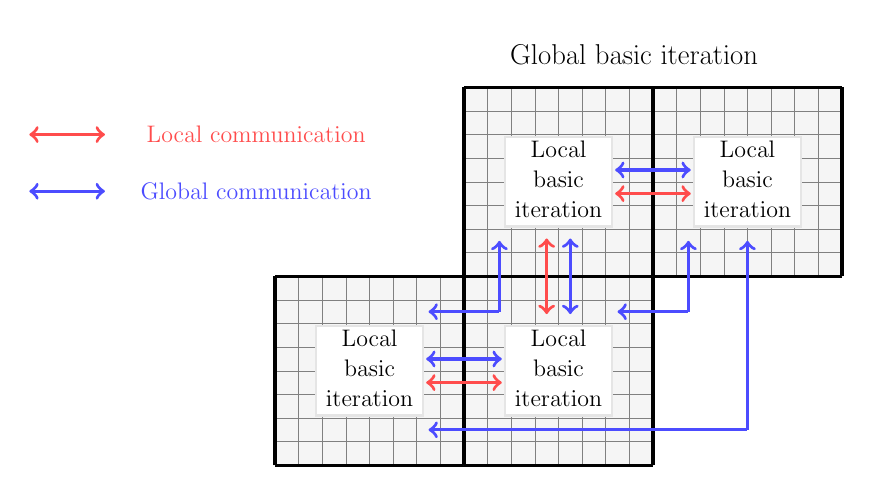
\begin{tikzpicture}
[
scale=0.6,
every node/.style={scale=0.6},
Background/.style={rectangle,draw=black!04,fill=black!04, thin, minimum size = 4 cm},
Obstruction/.style={rectangle,draw=black!70,fill=black!40, very thick, minimum size=1cm},
GlobalBorder/.style={-.,draw=black!100,  thin},
Finegrid/.style={step=0.5cm,gray,very thin},
Thickline/.style={-,draw=black!100,fill=black!02, very thick},
Thinline/.style={draw=black!100,fill=black!02, very thin},
Ball/.style={circle, draw=black!40, fill=red!20, thin, minimum size=3.5mm},
Circle/.style={circle,draw=black!40,fill=black!06,thin,minimum size=35.5mm},
Rectangle/.style={rectangle,draw=black!10,fill=white,inner xsep=0pt, inner ysep=0pt,},
Box/.style= {very thin, rectangle, inner xsep=10pt, inner ysep=10pt,},
ComRedArrow/.style= {very thick, draw=red!70,},
ComBlueArrow/.style= {very thick, draw=blue!70,},
DotArrow/.style= {<-, thick, dotted, draw=black!70,},
DotLine/.style= {very thick, dotted, draw=black!70,},
]

%\draw[GlobalBorder, fill=black!10] (-1.2,-1.2)--(13.2,-1.2)--(13.2,9.2)--(-1.2,9.2)--(-1.2,-1.2);
\node [Box, black] (box) at (7.6,8.7){\LARGE Global basic iteration};

\node[Background] at (  2,2) {};
\node[Background] at (  6,2) {};
\node[Background] at (  6,6) {};
\node[Background] at (10,6) {};

\node[Obstruction] at (2,2) {};

\draw[Finegrid] (0,0) grid (  8,4);
\draw[Finegrid] (4,4) grid (12,8);

\draw[Thickline] (0,0)--(  8,0);
\draw[Thickline] (4,8)--(12,8);
\draw[Thickline] (0,4)--(  4,4);
\draw[Thickline] (8,4)--(12,4);

\draw[Thickline] (  0,0)--(  0,4);
\draw[Thickline] (  4,8)--(12,8);
\draw[Thickline] (  4,4)--(  4,8);
\draw[Thickline] (  8,0)--(  8,4);
\draw[Thickline] (12,4)--(12,8);

\draw[Thickline] (4,0)--(4,4);
\draw[Thickline] (4,4)--(8,4);
\draw[Thickline] (8,4)--(8,8);

\node[Rectangle] at (  2,2.0) {\Large \begin{tabular}{c} Local \\ basic \\iteration \end{tabular}};
\node[Rectangle] at (  6,2.0) {\Large \begin{tabular}{c} Local \\ basic \\iteration \end{tabular}};
\node[Rectangle] at (  6,6.0) {\Large \begin{tabular}{c} Local \\ basic \\iteration \end{tabular}};
\node[Rectangle] at (10,6.0) {\Large \begin{tabular}{c} Local \\ basic \\iteration \end{tabular}};

\draw[<->,ComRedArrow](3.2,1.75)--(4.8,1.75);
\draw[<->,ComRedArrow](5.75,3.2)--(5.75,4.8);
\draw[<->,ComRedArrow](7.2,5.75)--(8.8,5.75);

\draw[<->,ComBlueArrow](3.2,2.25)--(4.8,2.25);
\draw[<->,ComBlueArrow](6.25,3.2)--(6.25,4.8);
\draw[<->,ComBlueArrow](7.2,6.25)--(8.8,6.25);

\draw[<-, ComBlueArrow](3.25,3.25)--(4.75,3.25);
\draw[->, ComBlueArrow](4.75,3.25)--(4.75,4.75);
\draw[<-, ComBlueArrow](7.25,3.25)--(8.75,3.25);
\draw[->, ComBlueArrow](8.75,3.25)--(8.75,4.75);
\draw[<-, ComBlueArrow](3.25,0.75)--(10,0.75);
\draw[->, ComBlueArrow](10.0,0.75)--(10,4.75);
%

\draw[<->,ComRedArrow](-5.2,7.0)--(-3.6,7.0);
\node [Box,red!70] (box) at (-0.4,7.0){%
    \begin{minipage}{0.56\textwidth}
    \begin{center}
        {\Large Local communication}
    \end{center}
    \end{minipage}};
    
\draw[<->,ComBlueArrow](-5.2,5.8)--(-3.6,5.8);
\node [Box,blue!70] (box) at (-0.4,5.8){%
    \begin{minipage}{0.56\textwidth}
    \begin{center}
        {\Large Global communication}
    \end{center}
    \end{minipage}};

\end{tikzpicture}

\caption{Inner core of \scarc{} consisting of a nested combination of a global data-parallel basic iteration defined on a global Poisson-matrix for the entire domain with mesh-wise preconditioning by local basic iterations.} 
\label{FIG_default_basic}
\end{center}
\end{figure}

The global basic iteration is distributed over the individual sub-meshes and serves to best possibly map the global dependencies. Since the matrix-vector products therein are related to the global Poisson-matrix and are only computed in a data-parallel way, there are no more errors along the mesh interfaces related to the normal components of velocity. This fact represents the most significant difference to the mesh-wise default FFT solver. However, the computation of these globally consistent matrix-vector products requires the local communication of mutually required data between adjacent meshes. Furthermore, to check the convergence criterion for the global basic iteration, overall defect norms have to be computed which requires global communication between all meshes as well.

Imbedded in this surrounding global basic iteration, the individual meshes perform their own local basic iterations until a predefined local stopping criterion has been reached. However, the respective local results are not used as solutions for their own, but only to correct the global solution and to guarantee a sufficiently high degree of local accuracy.  In particular, the preconditioners for the local basic iterations can be chosen individually corresponding to the local situation which of course requires appropriate strategies to properly balance the computational load across processors.

\subsubsection{Default 1-level generalizations of \scarc{}}
To improve the overall convergence speed, the global and local iterations are usually substituted by more efficient solution strategies as already mentioned above. The global iteration is typically replaced by a data-parallel CG- or MG-method. Apart from using the aforementioned globally defined matrix-vector products, these methods incorporate even more globally acting features such as global scalar-products in case of CG or an additional coarse grid problem in case of MG which furthermore contribute to a stronger global coupling.
In turn, there is a great freedom in the choice of the local solution techniques again. For example, the local iterations can be replaced by local MG-methods with different types of smoothing. Alternatively, optimized direct local solvers (according to the underlying discretization type) can be used leading to the exact solution of the local Poisson problems.

The resulting combination of global and local solvers can be used for structured and unstructured discretizations. In FDS the following two default variants for both cases are available.

\paragraph {Global structured discretization:}
The default variant for the structured case, simply abbreviated with \scarc{}, is illustrated in Figure \ref{FIG_default_scarc}. It can be called by setting {\ct SOLVER='SCARC'} in the {\ct \&PRES} name list and is based on a global, data-parallel CG method. Due to the structured discretization type, the mesh-wise preconditioning is done by local FFT methods based on the optimized CRAYFISHPAK package. But for exactly that reason, there still may be velocity penetration errors towards internal obstructions. Thus, this variant is  embedded into the already known pressure iteration. However, in contrast to the default FFT solver the velocity field is already correct along mesh interfaces and the pressure iteration only relates to internal obstructions.

\begin{figure}[h]
\begin{center}
\input{\tikzPath/multi_pipe_scarc.tex}
\caption{Default \scarc{} solver for a global structured discretization, consisting of a global data-parallel CG-method with mesh-wise preconditioning by local optimized FFT-methods, embedded in a pressure iteration to correct velocity penetration towards internal obstructions.} 
\label{FIG_default_scarc}
\end{center}
\end{figure}

\paragraph{Global unstructured discretization:}
The default variant for the unstructured case, simply abbreviated with \uscarc{}, is illustrated in Figure 
\ref{FIG_default_uscarc}. It can be called by setting {\ct SOLVER='USCARC'} in the {\ct \&PRES} name list
and is also based on a global data-parallel CG method. 
%
But due to the unstructured discretization type, the 
mesh-wise preconditioning can no longer be done by local FFT's, but local $LU$-decompositions are used instead which are based on the optimized {\tt PARDISO} solver of the Intel\textsuperscript{\textregistered} Math Kernel Library. Apart from the already correct transitions of the velocity field along mesh interfaces, the treatment of internal obstructions is also correct and no pressure iteration is needed at all.

Certainly, the use of the local $LU$-decompositions also requires additional memory.
However, these are only built and stored mesh-wise and do not act across the entire domain. Thus, the associated storage requirements seem to be acceptable or do at least not grow with increasing number of meshes. Nevertheless, as already mentioned, the local $LU$'s are not as efficient as the local FFT's, such that unstructured alternatives are currently being developed here.

\begin{figure}[h]
\begin{center}
\input{\tikzPath/multi_pipe_uscarc.tex}
\caption{Default \uscarc{} solver for a global unstructured discretization, consisting of a global data-parallel CG-method with mesh-wise preconditioning by local optimized $LU$-decompositions.} 
\label{FIG_default_uscarc}
\end{center}
\end{figure}

\subsubsection{Further multi-level generalizations of \scarc{}}
The \scarc{} variants shown so far were only defined on one single grid level, namely the fine level on which FFT and UGLMAT  are also built. However, a very important generalization is based on the use of additional coarser grid leves, which basically can contribute to a much better global coupling. The two most important multi-level representatives of ScaRC are presented below.

\paragraph{\scarcmultigrid{}:}
A special variant for structured discretizations, \scarcmultigrid{}, is based on the use of a global MG-method instead of the CG-method.
As illustrated in Figure \ref{FIG_default_scarc_mg} for the {\ct poisson2d} geometry, it not only uses one fine grid level, but a complete hierarchy of levels with increasingly coarser degree of grid resolution. The total possible number of levels depends on the grid resolution.
All levels work together in a well tuned choreography to finally produce a common global solution. 
Due to the structured nature of discretization an additional surrounding pressure iteration is used which, however, only relates to the internal obstructions as for \scarc{}.

\newpage
The combination of approximate solutions on the different refinement levels (based on a small number of SSOR-preconditioned basic iterations each) with an exact solution on the coarse grid level (based on a suitable direct solver), provides a much stronger global coupling which is reflected in significantly better convergence rates as can be seen for many test cases. Certainly, the computational effort is increased at the same time, which has to be set in relation to the resulting gain of numerical efficiency.


\begin{figure}[h]
\begin{center}
%--------------------------------------------------------------------------------------------------------------------
% Right lower picture: Unstructured grid
%--------------------------------------------------------------------------------------------------------------------
\begin{center}
\begin{tikzpicture}
[
 scale=0.62,
 ],
%
\node[inner sep=0pt] at (0,0)
 {\includegraphics[width=.45\textwidth]{./figures/mg_method_dashed.png}};

\foreach \y in {0,1,2} {
   \pgfmathsetlengthmacro{\ypos}{(\y*2.3-3+0.7)*1cm}
   \node at (-7,\ypos) { \small Level \y }; 
}

\draw [->, dashed] (0,-4) -- (0,-5) -- (8,-5) -- (8,5) -- (0,5) -- (0,4);
\node at (4,5.5) { \small Pressure iteration }; 

\def\xposC{-15.5}
\def\yred{2.5}
\def\yblue{1.5}
\node[text=red, anchor=west] (RED) at (\xposC,\yred) { \footnotesize Local communication }; 
\draw [<->, color=red, very thick] ($ (RED.west) - (1,0) $) -- (RED.west);
\node[text=blue, anchor=west] (BLUE) at (\xposC,\yblue) { \footnotesize Global communication }; 
\draw [<->, color=blue, very thick] ($ (BLUE.west) - (1,0) $) -- (BLUE.west);

\def\xposG{-13.5}
\node[inner sep=0pt] (TRANS) at (\xposG,-1.1)
 {\includegraphics[scale=0.7]{./figures/mg_transfer.png}};
\node at ($(TRANS.south) - (0,0.5)$) { \footnotesize Grid transfer }; 

\end{tikzpicture}
\end{center}
%

\caption{Alternative version \scarcmultigrid{} for a global structured discretization, consisting of a global data-parallel MG-method with mesh-wise SSOR-smoothing, embedded in a pressure iteration to correct velocity penetration towards internal obstructions.} 
\label{FIG_default_scarc_mg}
\end{center}
\end{figure}

\paragraph{\scarctwolevel{}:}
Another structured multi-level variant, \scarctwolevel{}, is based on the use of exactly two grid levels.
In the same way as the default \scarc{} version, it performs a global CG-method on the finest grid level. In addition, exactly one further level with a coarser degree of resolution is used, on which the associated restricted problem is solved by a globally acting solver (mostly a direct one) with the highest possible accuracy. This level may consist of one or more coarsenings of the finest grid level whereby the domain decomposition itself is the coarsest possible level. As for all structured \scarc{} variants, a surrounding pressure iteration is used which only relates to the internal obstructions.

Again, both fine and coarse grid levels closely work together to finally produce a common solution which incorporates a much higher level of global coupling compared to the 1-level counterpart due to the additional coarse information.  

A graphical representation for \scarctwolevel{} is not used at this point. However, as an example for the {\ct poisson2d} geometry, Level 2 and Level 0 from Figure \ref{FIG_default_scarc_mg} could be taken as fine and coarse grid level for the \scarctwolevel{} variant.

\newpage
\subsubsection{Preliminary assessment and application notes}
In the light of the above discussions, the acronym \scarc{} stands for:
\begin{itemize}
\item {\it {\bf Sca}lable}, because the number of global and local iterations can be varied,
\item {\it {\bf R}ecursive}, since it can be applied recursively to more than 2 levels with different refinements,
\item {\it {\bf C}lustering}, since neighboring meshes can be merged into larger clusters with special treatment.
\end{itemize}
Due to the complexity of the topic, an all-encompassing presentation was not possible here, but only a rough overview of the basic functionality and the most important representatives should be given. 
A detailed description of the underlying algorithmic concepts can be found in~\cite{Kilian:2001, Kilian:1998, Goeddeke:2010, Wobker:2010}.

In order to access the most recent version of \scarc{} it is necessary to download a clone of the FDS repository and to compile the code yourself. Please note, that there are still some limitations in the use of \scarc{} which actually correspond to those for  \uglmat{}, namely that it can only be applied for non-overlapping, non-stretched meshes at the same refinement level. 
%
While the use of an overlapping decomposition isn't necessary by design, the other two restrictions are only temporary in nature and corresponding enhancements are currently in progress. 

Clearly, \scarc{} is not a pure black-box solver and its application requires a careful assessment of the underlying problem characteristics. However, its major advantage is that it allows a very diverse combination of different components with regard to the selection of the global solvers (CG, MG or combinations of both), the local solvers (from simple basic iterations to highly optimized MG) and the local accuracy requirements (from gaining only one digit up to machine precision) such that any available information about the underlying problem can be exploited.

With respect to the choice of the local solvers, there is great potential for further variations and optimization. 
In the most recent test calculations, the FFT's have turned out to be the fastest local solvers so far. In particular, they are comprehensively faster than the local $LU$'s which may lead to the following unexpected circumstances: Although \uscarc{} doesn't need the pressure iteration (due to the correct treatment of internal obstructions) its runtime may be longer than that of \scarc{} explicitly performing the pressure iteration, namely just in such cases where only a small number of pressure iterations are needed to drive the penetration error below the specified tolerance. This imbalance is to be addressed by developing more efficient local solvers for the unstructured case.

%There are much more other variants which can be selected by further \scarc{} related parameters in the {\ct \&PRES} namelist. But many of these variants are not yet finally tuned and some detailed knowledge about the underlying algorithms is still necessary. Once these variants are mature, they will be made available in a default version along with a detailed description.

In conclusion it must be pointed out that \scarc{} is still in a beta development state.
Test calculations for a large number of cases have shown that it basically is able to achieve a high level of accuracy.
This is mostly due to the fact that a global discretization is used so that the correct velocity field along inner mesh interfaces is calculated and no additional pressure iteration is needed there. In case of the unstructured variant \uscarc{}, the penetration errors towards inner obstructions are also eliminated. 

However, especially in case of longer lasting validation cases, it has also been observed that the previous runtimes are not yet optimal. This remaining weakness is mainly based on the fact that the focus of the development has been on the fundamental algorithmic correctness of the individual solution components and less on runtime performance so far. Nevertheless, there is still a great potential for runtime improvements and corresponding improvements are currently in progress.
